\section{Appendix A}
\subsection{Incomplete CFD Models}
In addition to the CFD models and results discussed above, several other, higher fidelity models were attempted. These models were not usable as discrepancies and physically impossible data was found in the outputs. For the sake of completeness, the most complete model is briefly discussed here.

\subsubsection{Cowl and Diffuser Model}
The model that was closest to being usable simulated both a cowl and a subsonic diffuser. Figure \ref{fig:InletSurf} displays the 2D surface imported into Ansys$\copyright$. The boundary conditions used for the simulation are also displayed in Fig. \ref{fig:InletBCs}.

\begin{figure}[H]
\centering
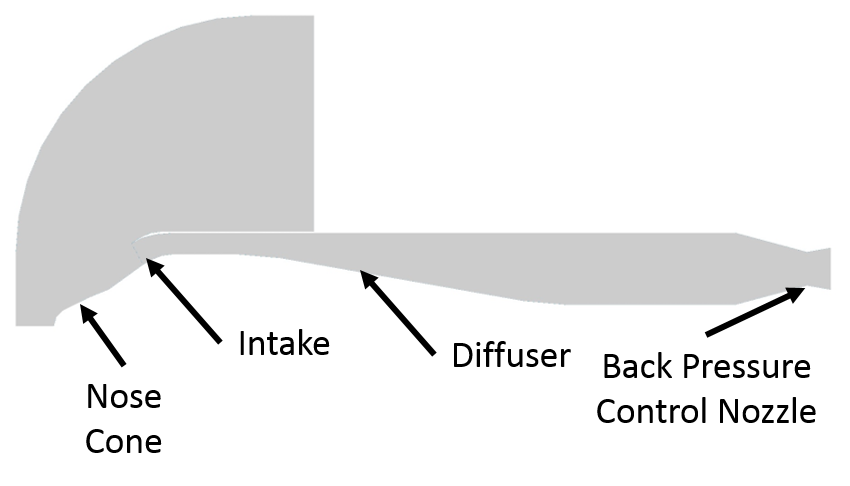
\includegraphics[width=.7\textwidth]{JWE_Figures/CFD_Surface.png}
\caption{Inlet surface used to generate axisymmetric grid in CFD}
\label{fig:InletSurf}
\end{figure}

\begin{figure}[H]
\centering
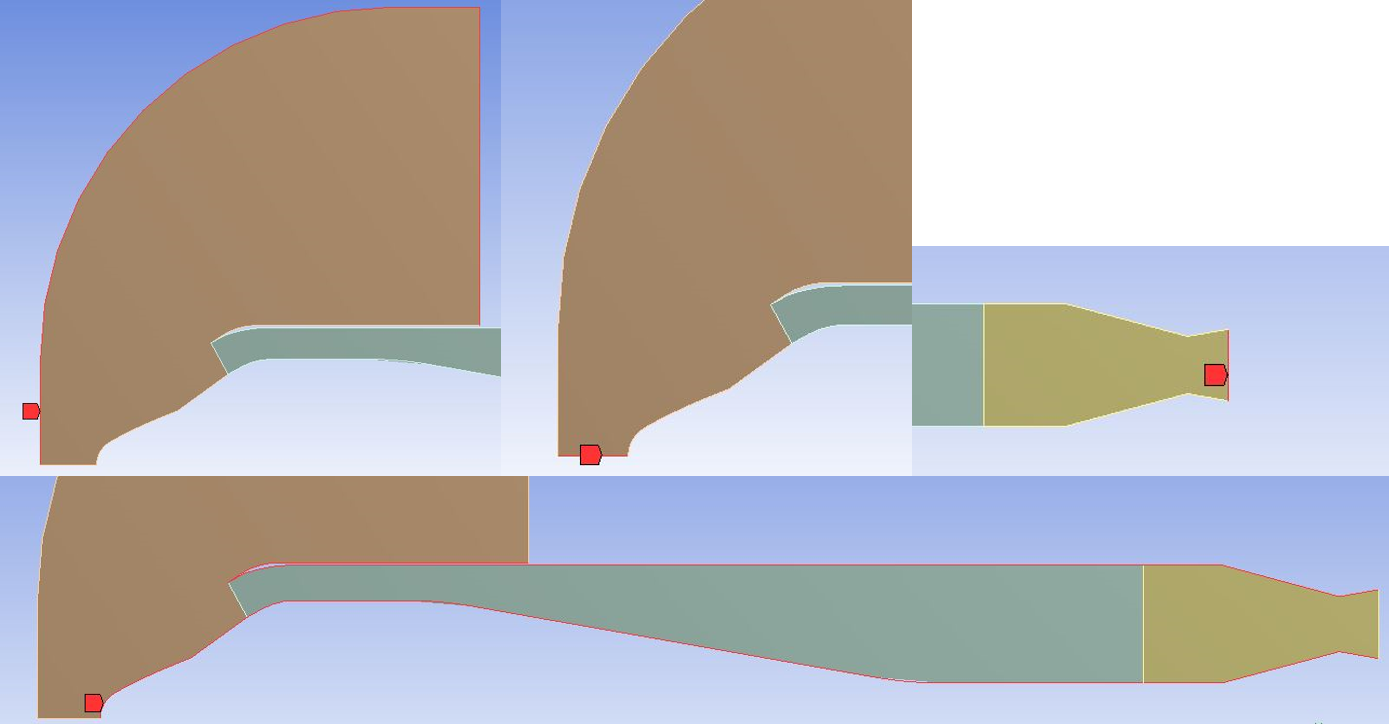
\includegraphics[width=1.0\textwidth]{JWE_Figures/BC_Group.png}
\caption{Boundary conditions for CFD study. Top left: Pressure far field. Top middle: Axis for revolution. Top right: Pressure out. Bottom: Wall}
\label{fig:InletBCs}
\end{figure}

This model had the advantage of (theoretically) simulate the full regime of flow through the inlet. This would be achieved by varying the nozzle diameter on the back end of the geometry to adjust the static pressure and mass flow through the inlet. This would mean that instead of interpolating the cane curves, as was done, the CFD calculations would have been able to fully calculate them. However, examining the data for several Mach 2.5 cases, the data was suggesting that there was more mass flow through the nozzle than is physically possible given the capture area. The maximum flow that the inlet can ingest is 21 kg/s. Some cases of were predicting up to 25 kg/s. In addition, instead of reaching a max flow rate at a critical pressure then staying constant for lower back pressures, the predicted mass flows were scattered with no clear pattern. See Fig. \ref{fig:FailedCane} for the output data of these cases.

\begin{figure}[H]
\centering
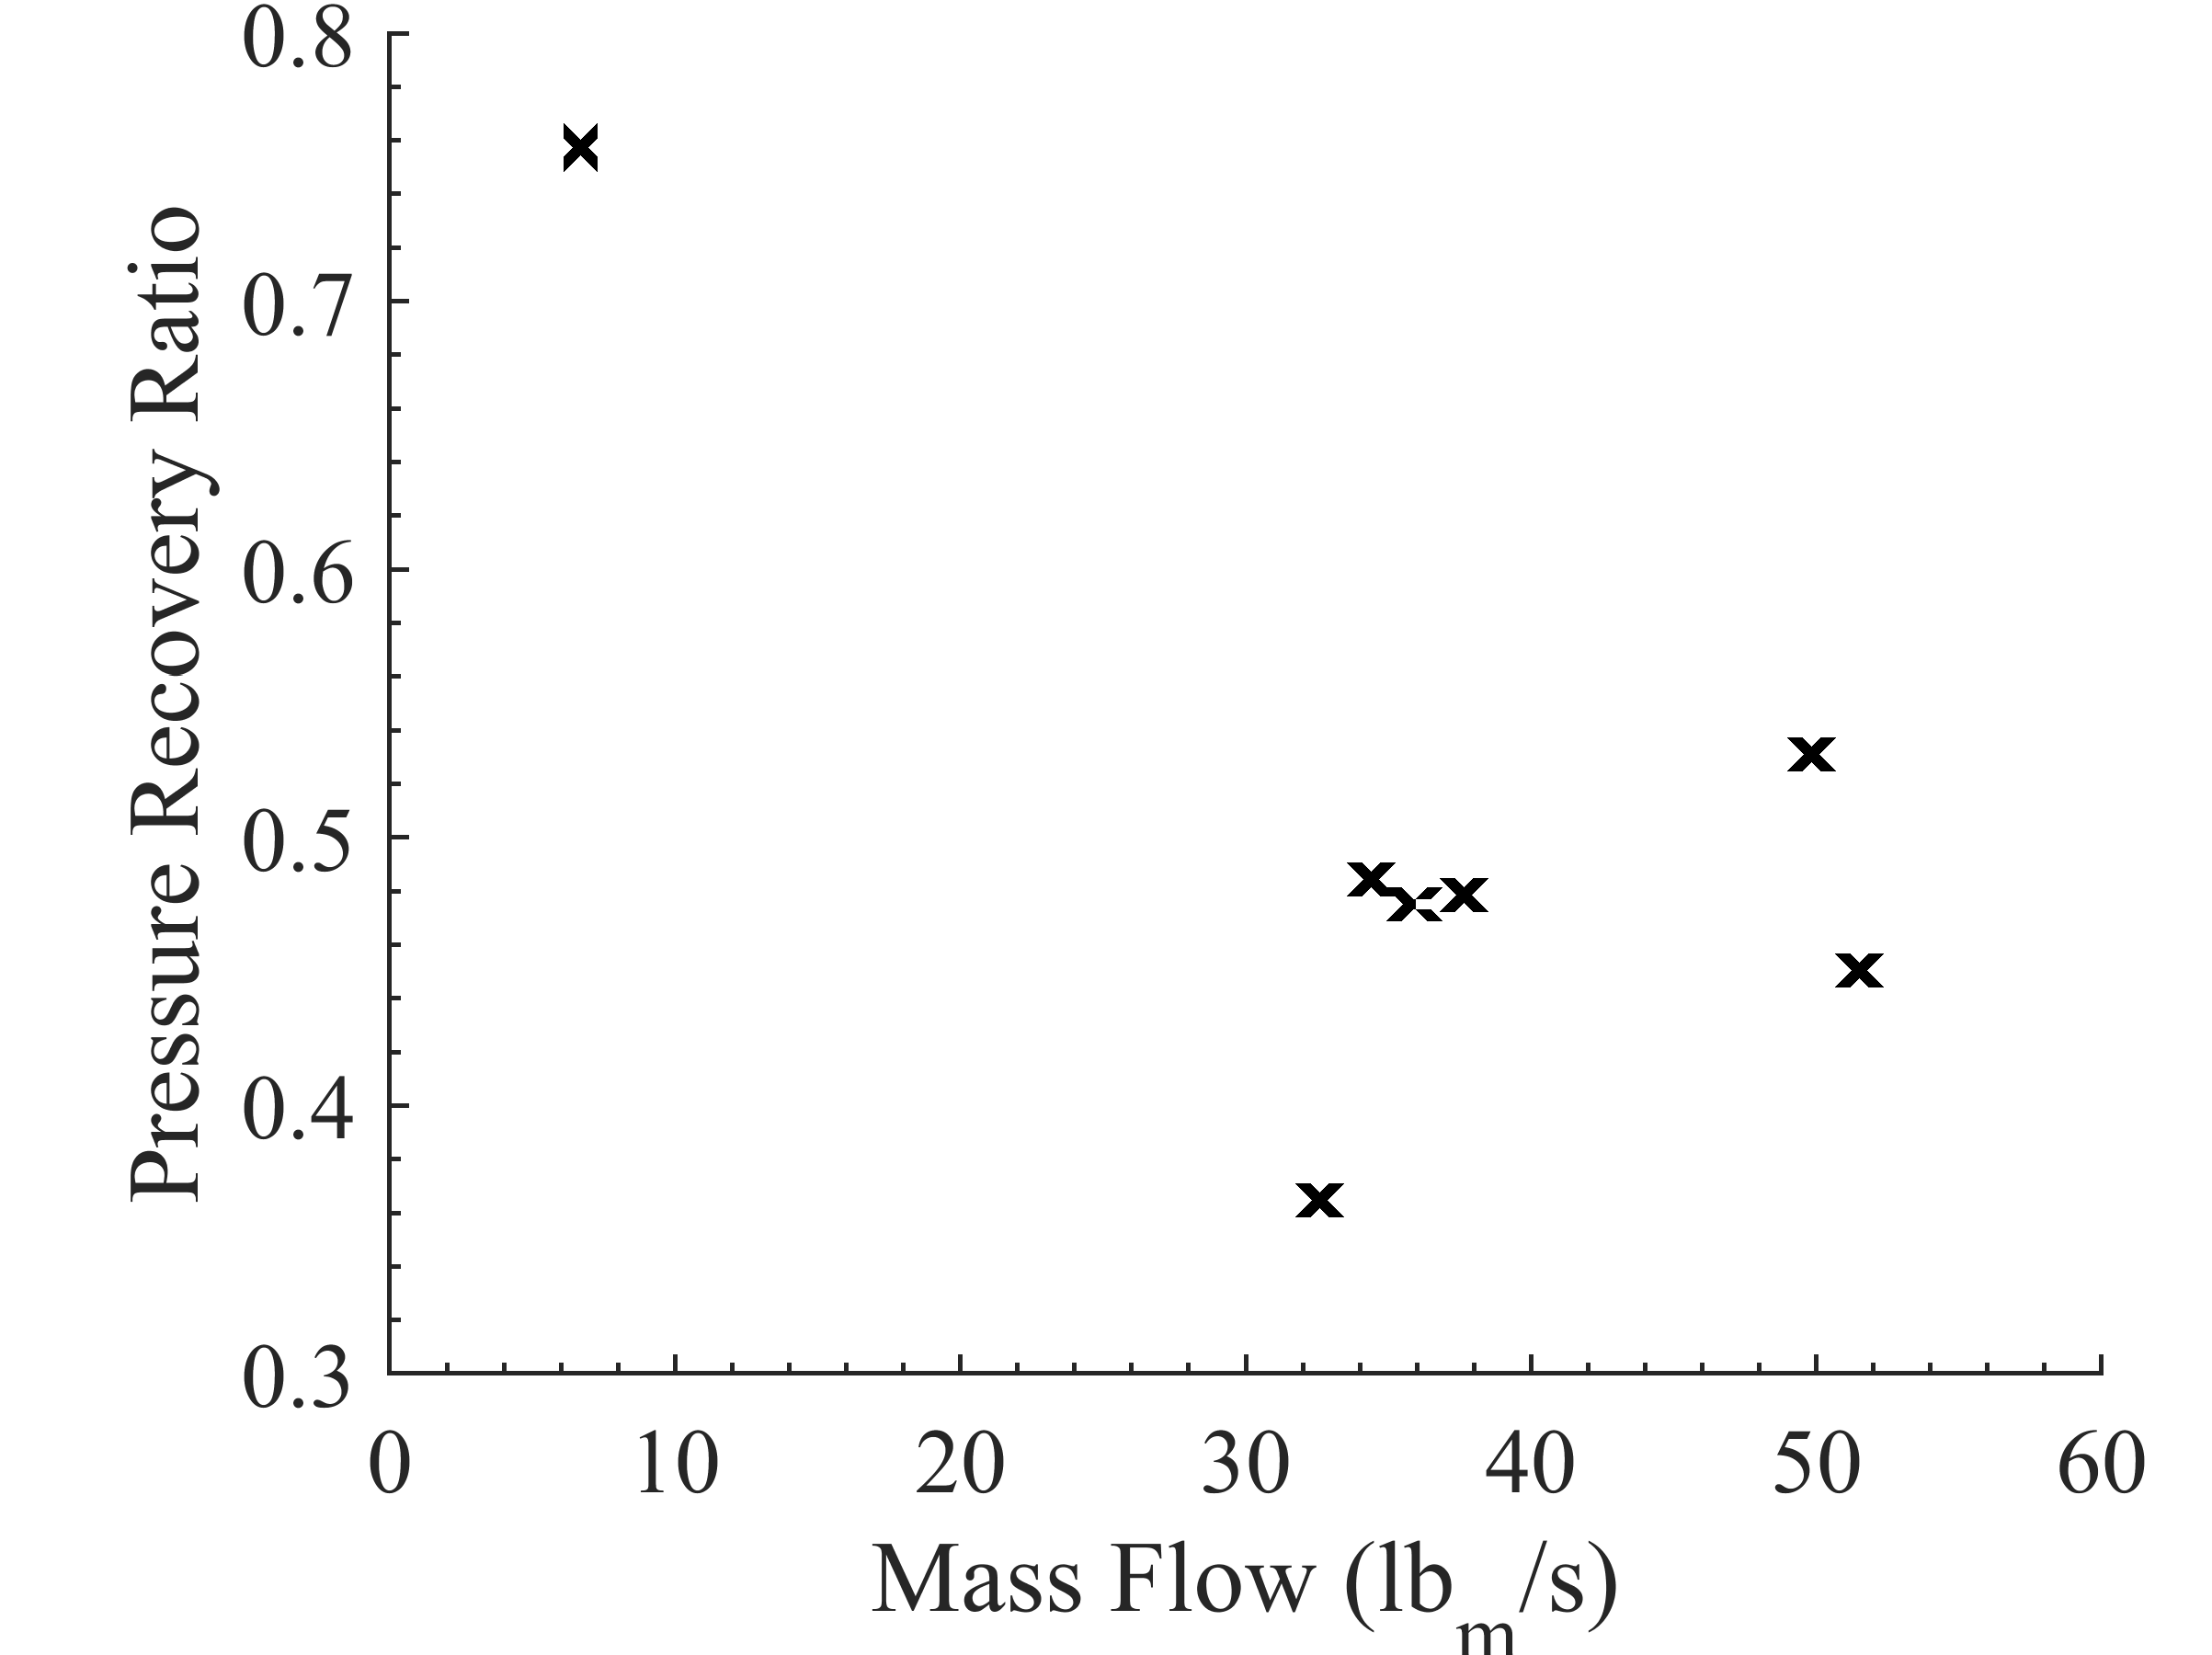
\includegraphics[width=.5\textwidth]{JWE_Figures/P_Recov_2_5.png}
\caption{CFD data of Mach 2.5 cases }
\label{fig:FailedCane}
\end{figure}

From the onset, it was a struggle to get the solution to not crash, let alone converge on a single answer. Numerous combinations of pressure and density based solvers were used with varying orders of solution methods and damping factors. No solution method more accurate than first order upwind ever returned a non-crashed computation. The likely cause of this failure was the unsteady nature of the flow within the inlet. There appeared to be separated flow on the subsonic diffuser, creating recirculating zones that are inherently unsteady. Also, ramjets are known to "buzz" in steady state in certain pressure ranges. This unsteady behavior could easily destabilize the solution and make a computation meaningless. Moving forward, the inlet will need to be examined by a knowledgeable CFD engineer, as both unsteady and 3D methods will need to be used to establish a more complete operational behavior.

The two contour plots bellow show the Mach number and pressure profiles within the inlet. The Mach contour shows the recirculation and separation on the diffuser that likely made the solution difficult. The pressure plot also seams to show slightly circular regions of increased pressure. These are likely indications of artifacts or point discontinuities within the calculations.

\begin{figure}[H]
\centering
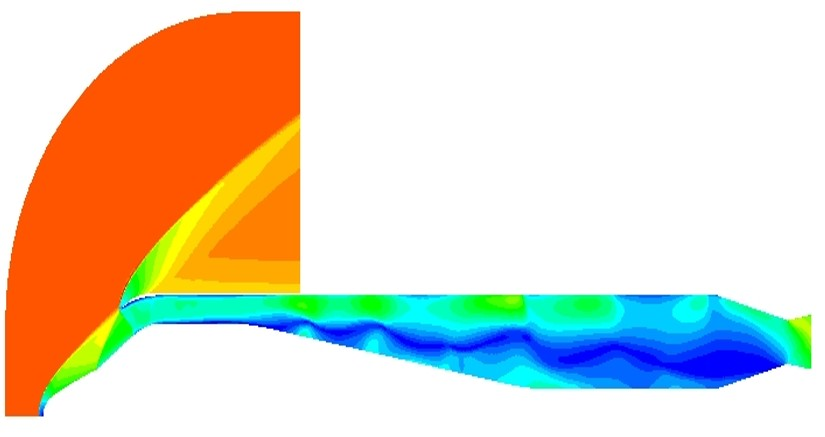
\includegraphics[width=1.0\textwidth]{JWE_Figures/Critical_Mach_2_5.jpg}
\caption{Relative Mach number contour within the inlet at Mach 2.5 free stream}
\label{fig:InletMach}
\end{figure}

\begin{figure}[H]
\centering
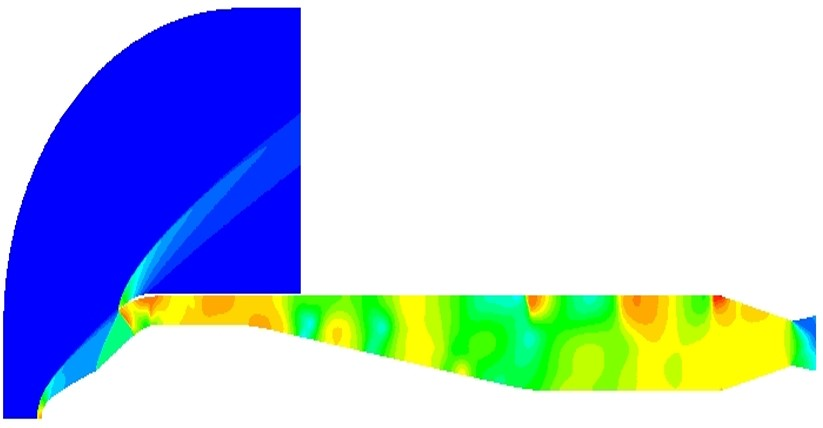
\includegraphics[width=1.0\textwidth]{JWE_Figures/Critical_Mach_2_5_Pressure.jpg}
\caption{Relative pressure contour within the inlet at Mach 2.5 free stream}
\label{fig:InletPSI}
\end{figure}

\subsubsection{Grid Convergence Study}

As is the norm with CFD computations, a grid convergence study was conducted for the failed model. The study seemed to suggest that the computation was converging on a single answer initially. However, when the non-physical data was discovered later, re-runs of the same grid studies with identical solution methods, starting states, and iterations resulted in different answers.

Figure \ref{fig:InletMeshDrivers} below shows the meshing setup for the grid study. A 'base size element was selected, with smaller base elements used for increased resolution. That base element size, or a fraction of it, was then used to influence the local element sizes in order to refine the mesh around important flow points.

\begin{figure}[H]
\centering
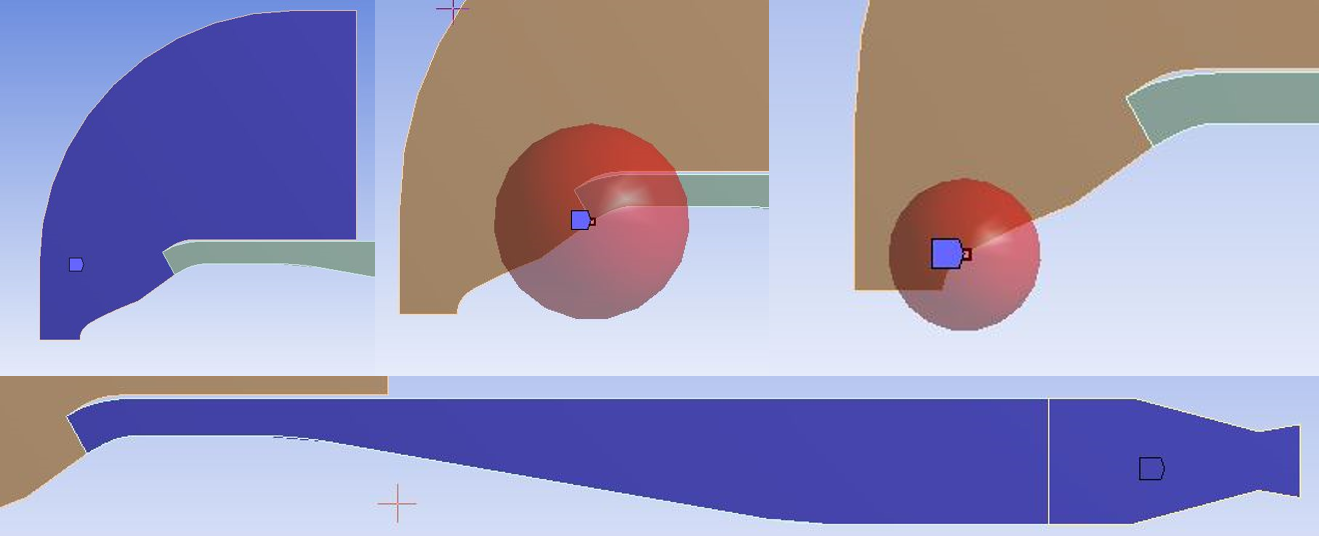
\includegraphics[width=1.0\textwidth]{JWE_Figures/MeshGroup.png}
\caption{Mesh setup for grid convergence study showing mesh type and size factor. Top Left: Face sizing, base size = 1. Top middle: Influence sphere, base size = 1/4.  Top right: Influence sphere, base size = 1/4. Bottom: Face sizing, base size = 1/2. }
\label{fig:InletMeshDrivers}
\end{figure}